
\documentclass[border=10pt, 12pt]{standalone}
\usepackage[svgnames]{xcolor}
\usepackage{amsmath}
\usepackage{pgfplots}
\pgfplotsset{compat=newest}
\usepackage[sfdefault]{FiraSans}
\usepackage{FiraMono}
\renewcommand*\familydefault{\sfdefault}
\begin{document}
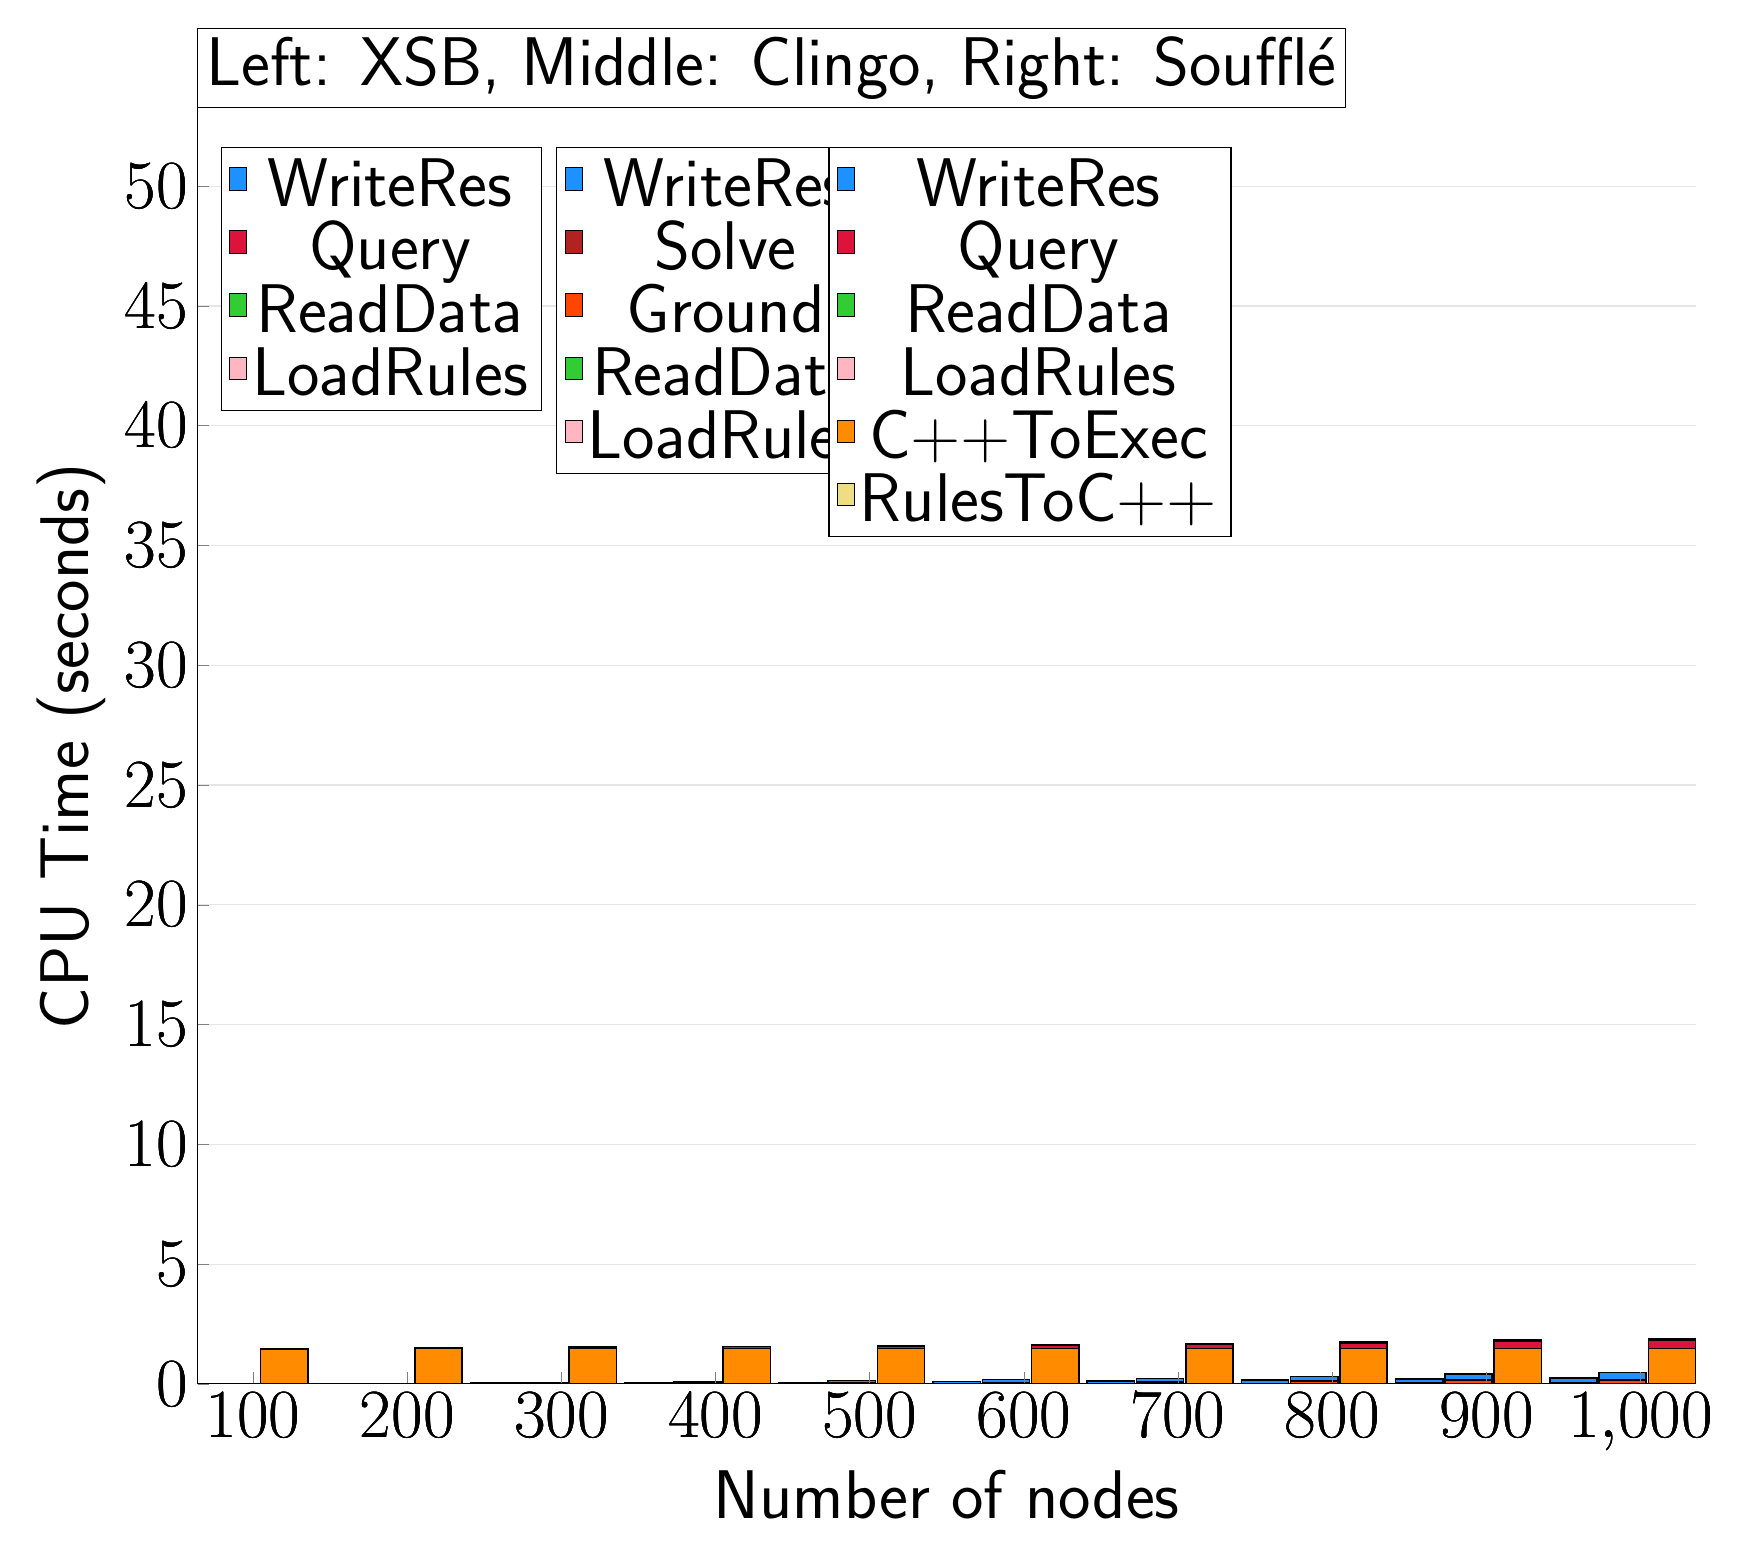
\begin{tikzpicture}
                        \begin{axis}[bar shift=-24.3pt, 
   ybar stacked,
   width=1.7\textwidth,
   bar width=0.6cm,
   ymajorgrids, tick align=inside,
   major grid style={draw=gray!20},
   xtick=data,
   ymin=0, ymax=53.25004,
   axis x line*=bottom,
   axis y line*=left,
   enlarge x limits=0.04,
   legend style={
       at={(0.23, 0.97)},
       anchor=north east,
       legend columns=1,
       font=\Huge,
   },
   ylabel={CPU Time (seconds)},
   xlabel={Number of nodes},
   label style={font=\Huge},
   tick label style={font=\Huge},
]
\addlegendimage{fill=DodgerBlue, draw=black, line width=0.2pt}
\addlegendentry{WriteRes}
\addlegendimage{fill=Crimson, draw=black, line width=0.2pt}
\addlegendentry{Query}
\addlegendimage{fill=LimeGreen, draw=black, line width=0.2pt}
\addlegendentry{ReadData}
\addlegendimage{fill=LightPink, draw=black, line width=0.2pt}
\addlegendentry{LoadRules}
\addplot +[fill=LightPink, draw=black, line width=0.55pt] coordinates {
(100, 0.0005482)
(200, 0.0005519999999999996)
(300, 0.0005482000000000004)
(400, 0.0005483999999999995)
(500, 0.0005505999999999999)
(600, 0.0005507999999999999)
(700, 0.0005466000000000002)
(800, 0.0005487999999999998)
(900, 0.0005509999999999996)
(1000, 0.0005492000000000006)
};
\addplot +[fill=LimeGreen, draw=black, line width=0.55pt] coordinates {
(100, 0.00025760000000000024)
(200, 0.0003990000000000004)
(300, 0.0005426)
(400, 0.0007156000000000005)
(500, 0.0008346000000000002)
(600, 0.0009781999999999998)
(700, 0.0011372)
(800, 0.0013024)
(900, 0.0014874)
(1000, 0.001579)
};
\addplot +[fill=Crimson, draw=black, line width=0.55pt] coordinates {
(100, 0.00040300000000000015)
(200, 0.0014156)
(300, 0.0029888000000000002)
(400, 0.005664000000000001)
(500, 0.0082652)
(600, 0.0115256)
(700, 0.0157172)
(800, 0.021204)
(900, 0.0281234)
(1000, 0.03235400000000001)
};
\addplot +[fill=DodgerBlue, draw=black, line width=0.55pt] coordinates {
(100, 0.0024879999999999998)
(200, 0.009171000000000002)
(300, 0.0193438)
(400, 0.03696000000000001)
(500, 0.053424400000000004)
(600, 0.07475380000000001)
(700, 0.10297540000000001)
(800, 0.137359)
(900, 0.1804556)
(1000, 0.20352640000000002)
};
\end{axis}

\begin{axis}[bar shift=-6.5pt, 
   ybar stacked,
   width=1.7\textwidth,
   bar width=0.6cm,
   ymajorgrids, tick align=inside,
   major grid style={draw=none},
   xtick=data,
   ymin=0, ymax=53.25004,
   axis x line*=none,
   axis y line*=none,
   enlarge x limits=0.04,
   legend style={
       at={(0.454, 0.97)},
       anchor=north east,
       legend columns=1,
       font=\Huge,
   },
   label style={font=\Huge},
   tick label style={font=\Huge},
]
\addlegendimage{fill=DodgerBlue, draw=black, line width=0.2pt}
\addlegendentry{WriteRes}
\addlegendimage{fill=FireBrick, draw=black, line width=0.2pt}
\addlegendentry{Solve}
\addlegendimage{fill=OrangeRed, draw=black, line width=0.2pt}
\addlegendentry{Ground}
\addlegendimage{fill=LimeGreen, draw=black, line width=0.2pt}
\addlegendentry{ReadData}
\addlegendimage{fill=LightPink, draw=black, line width=0.2pt}
\addlegendentry{LoadRules}
\addplot +[fill=LightPink, draw=black, line width=0.55pt] coordinates {
(100, 0.0)
(200, 0.0)
(300, 0.0)
(400, 0.0)
(500, 0.0)
(600, 0.0)
(700, 0.0)
(800, 0.0)
(900, 0.0)
(1000, 0.0)
};
\addplot +[fill=LimeGreen, draw=black, line width=0.55pt] coordinates {
(100, 0.0)
(200, 0.0)
(300, 0.0)
(400, 0.0)
(500, 0.0)
(600, 0.0)
(700, 0.0)
(800, 0.0)
(900, 0.0)
(1000, 0.0)
};
\addplot +[fill=OrangeRed, draw=black, line width=0.55pt] coordinates {
(100, 0.0)
(200, 0.0040000000000000036)
(300, 0.01200000000000001)
(400, 0.030000000000000027)
(500, 0.040000000000000036)
(600, 0.06)
(700, 0.08600000000000002)
(800, 0.11400000000000002)
(900, 0.15000000000000002)
(1000, 0.16800000000000004)
};
\addplot +[fill=FireBrick, draw=black, line width=0.55pt] coordinates {
(100, 0.0)
(200, 0.006000000000000005)
(300, 0.0040000000000000036)
(400, 0.0)
(500, 0.0)
(600, 0.0)
(700, 0.010000000000000007)
(800, 0.007999999999999974)
(900, 0.010000000000000009)
(1000, 0.01799999999999996)
};
\addplot +[fill=DodgerBlue, draw=black, line width=0.55pt] coordinates {
(100, 0.0020000000000000018)
(200, 0.0040000000000000036)
(300, 0.020000000000000018)
(400, 0.04999999999999999)
(500, 0.08999999999999997)
(600, 0.12)
(700, 0.13599999999999995)
(800, 0.1900000000000001)
(900, 0.248)
(1000, 0.28200000000000003)
};
\end{axis}

\begin{axis}[bar shift=11.3pt, 
   ybar stacked,
   width=1.7\textwidth,
   bar width=0.6cm,
   ymajorgrids, tick align=inside,
   major grid style={draw=none},
   xtick=data,
   ymin=0, ymax=53.25004,
   axis x line*=none,
   axis y line*=none,
   enlarge x limits=0.04,
   legend style={
       at={(0.69, 0.97)},
       anchor=north east,
       legend columns=1,
       font=\Huge,
   },
   label style={font=\Huge},
   tick label style={font=\Huge},
]
\addlegendimage{fill=DodgerBlue, draw=black, line width=0.2pt}
\addlegendentry{WriteRes}
\addlegendimage{fill=Crimson, draw=black, line width=0.2pt}
\addlegendentry{Query}
\addlegendimage{fill=LimeGreen, draw=black, line width=0.2pt}
\addlegendentry{ReadData}
\addlegendimage{fill=LightPink, draw=black, line width=0.2pt}
\addlegendentry{LoadRules}
\addlegendimage{fill=DarkOrange, draw=black, line width=0.2pt}
\addlegendentry{C++ToExec}
\addlegendimage{fill=LightGoldenrod, draw=black, line width=0.2pt}
\addlegendentry{RulesToC++}
\addplot +[fill=LightGoldenrod, draw=black, line width=0.55pt] coordinates {
(100, 0.0)
(200, 0.010000000000000002)
(300, 0.006000000000000001)
(400, 0.004000000000000001)
(500, 0.006000000000000001)
(600, 0.0020000000000000005)
(700, 0.004000000000000001)
(800, 0.006000000000000001)
(900, 0.010000000000000002)
(1000, 0.004000000000000001)
};
\addplot +[fill=DarkOrange, draw=black, line width=0.55pt] coordinates {
(100, 1.464)
(200, 1.46)
(300, 1.4659999999999997)
(400, 1.472)
(500, 1.462)
(600, 1.472)
(700, 1.472)
(800, 1.462)
(900, 1.464)
(1000, 1.472)
};
\addplot +[fill=LightPink, draw=black, line width=0.55pt] coordinates {
(100, 0.0001514)
(200, 0.00015040000000000002)
(300, 0.0001546)
(400, 0.00015780000000000001)
(500, 0.0001542)
(600, 0.0001528)
(700, 0.0001462)
(800, 0.0001468)
(900, 0.0001636)
(1000, 0.00015000000000000001)
};
\addplot +[fill=LimeGreen, draw=black, line width=0.55pt] coordinates {
(100, 0.0012070000000000002)
(200, 0.0019136000000000001)
(300, 0.00258)
(400, 0.0032714)
(500, 0.0040534)
(600, 0.0045808)
(700, 0.0048062)
(800, 0.0058878)
(900, 0.0066722000000000005)
(1000, 0.0072216)
};
\addplot +[fill=Crimson, draw=black, line width=0.55pt] coordinates {
(100, 0.0076554)
(200, 0.025887999999999994)
(300, 0.0465858)
(400, 0.0736136)
(500, 0.0991966)
(600, 0.13123279999999998)
(700, 0.17215160000000002)
(800, 0.22730540000000002)
(900, 0.294833)
(1000, 0.3347694)
};
\addplot +[fill=DodgerBlue, draw=black, line width=0.55pt] coordinates {
(100, 0.0016068000000000002)
(200, 0.0039464)
(300, 0.0063592)
(400, 0.0096974)
(500, 0.0139994)
(600, 0.0195154)
(700, 0.0264486)
(800, 0.0355302)
(900, 0.0463218)
(1000, 0.0526578)
};
\end{axis}


\node[anchor=south, draw, fill=white] at (rel axis cs:0.42,1) {\Huge Left: XSB, Middle: Clingo, Right: Soufflé};
\end{tikzpicture}
\end{document}
                    